\section{Labeling}
\label{sec:labeling}

Labels should have indicative prefixes - fig for Figures, sec for Sections, tab for Tables, eq for equations. Two labeling examples are given, for Figure \ref{fig:shapes} and for Table \ref{tab:experiment1_data}. To ensure quality, always use vector graphic images. 

\begin{figure}[ht!]
	\centering
		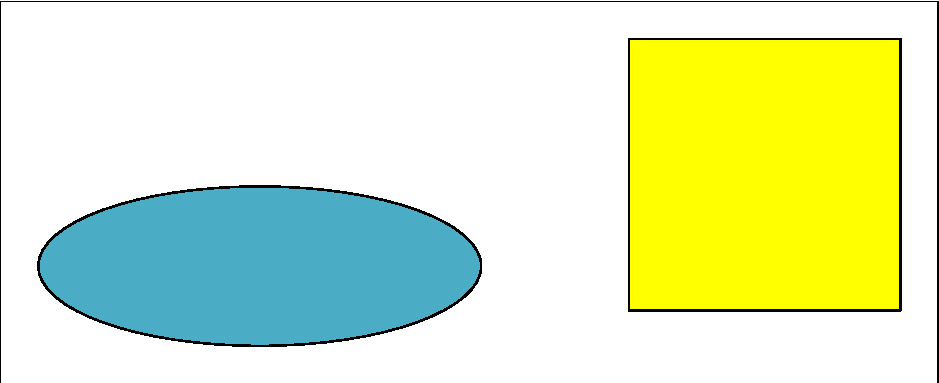
\includegraphics[width=0.7\linewidth]{shapes.pdf}
	\caption{Figure explanation goes here}
	\label{fig:shapes}
\end{figure}

\begin{table}[ht!]
	\centering
	\begin{tabular}{ccc}
		\toprule
		Station & $t_e [h]$ & $c_e^2$ \\
		\midrule
		1       & 1.5       & 1.5\\
		2       & 1.6       & 0.75\\
		\bottomrule
	\end{tabular}
	\caption{Table data description goes here}
	\label{tab:experiment1_data}
\end{table}

Bibitems should be labeled according to the first author surname and publication date, for example 'sewlal2014'. Useful resources on the topic of best practices in LaTeX are, for example, \cite{sewlal2014} and \cite{birotic2015}.


